\documentclass[12pt]{report}

\usepackage{setspace}
\setlength{\parindent}{4em}

\usepackage{fancyvrb}
\usepackage{graphicx}
\usepackage{geometry}

\geometry{letterpaper, portrait, margin=1in}

%%%Title Page%%%
\title{
  Lab 07
\bigbreak 4-bit UpDown Counter
}

\author{
{\normalsize
\begin{tabular}{l r r}
 & \textbf{Ryan Cruz} & \textbf{Zachary Davis}\\
\textbf{Category} & ryan.cruz25@uga.edu & zachdav@uga.edu\\
\hline
Pre-lab 						  & 50 & 50\\
In-lab Module \& Testbench Design & 50 & 50\\
In-lab Testbench Sim. \& Analysis & 50 & 50\\
In-lab FPGA Synthesis \& Analysis & 50 & 50\\
Lab Report Writing 				  & 50 & 50\\
\end{tabular}
}
}

\date{\bigskip
\today}
%%%%%%%%%%%%

\begin{document}
\maketitle

\section*{Lab Purpose}
	\paragraph{}
	The purpose of this lab is to implement a behavioral 4-bit up-down counter and interface it with the seven segment LED display using binary coded decimal, using knowledge from Lab03. The counter will count at 1 Hz, using the clock divider that we learned how to implement in the last lab. The counter has the ability to count up and down from 0 to 15. It wraps when it hits either boundary, and can be reset and paused with buttons on the board that we map using a module and \texttt{.ucf}.
\section*{Implementation Details}
	\subsection*{Pre-Lab Design}
		\paragraph*{Finite-State-Machine}
				\begin{center}
					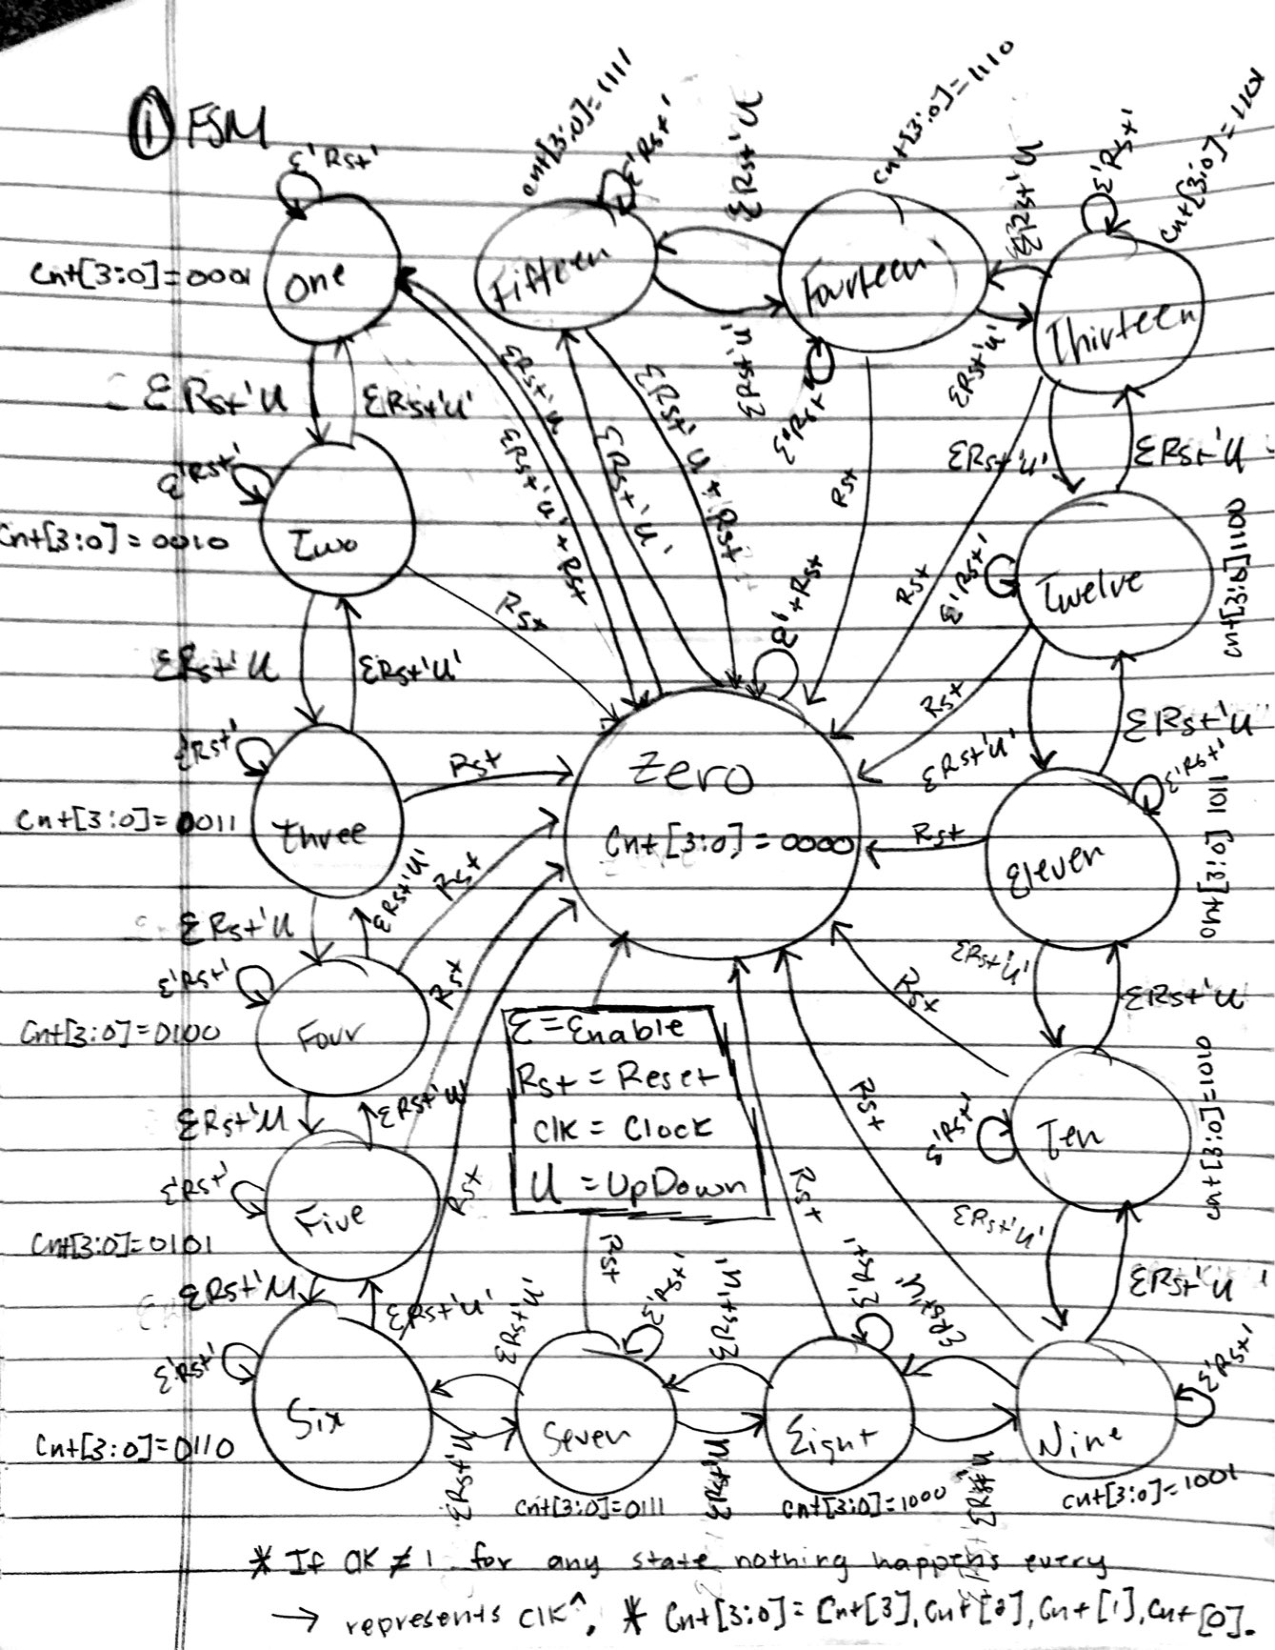
\includegraphics[scale=.5]{Prelab_7-page1.pdf}
				\end{center}
				\paragraph*{}This FSM shows our intended design for the following project.  
				If Enable is high and Rst is low then it counts up or down depending on the state 
				of the UpDown switch.  If Rst is high in any state it returns to Zero.  If Enable 
				is low and Rst is low then it remains in whatever states it was in.  The positive 
				clock edge is assumed to be true for ever equation.
		\paragraph*{Controller Design}

			\begin{center}
				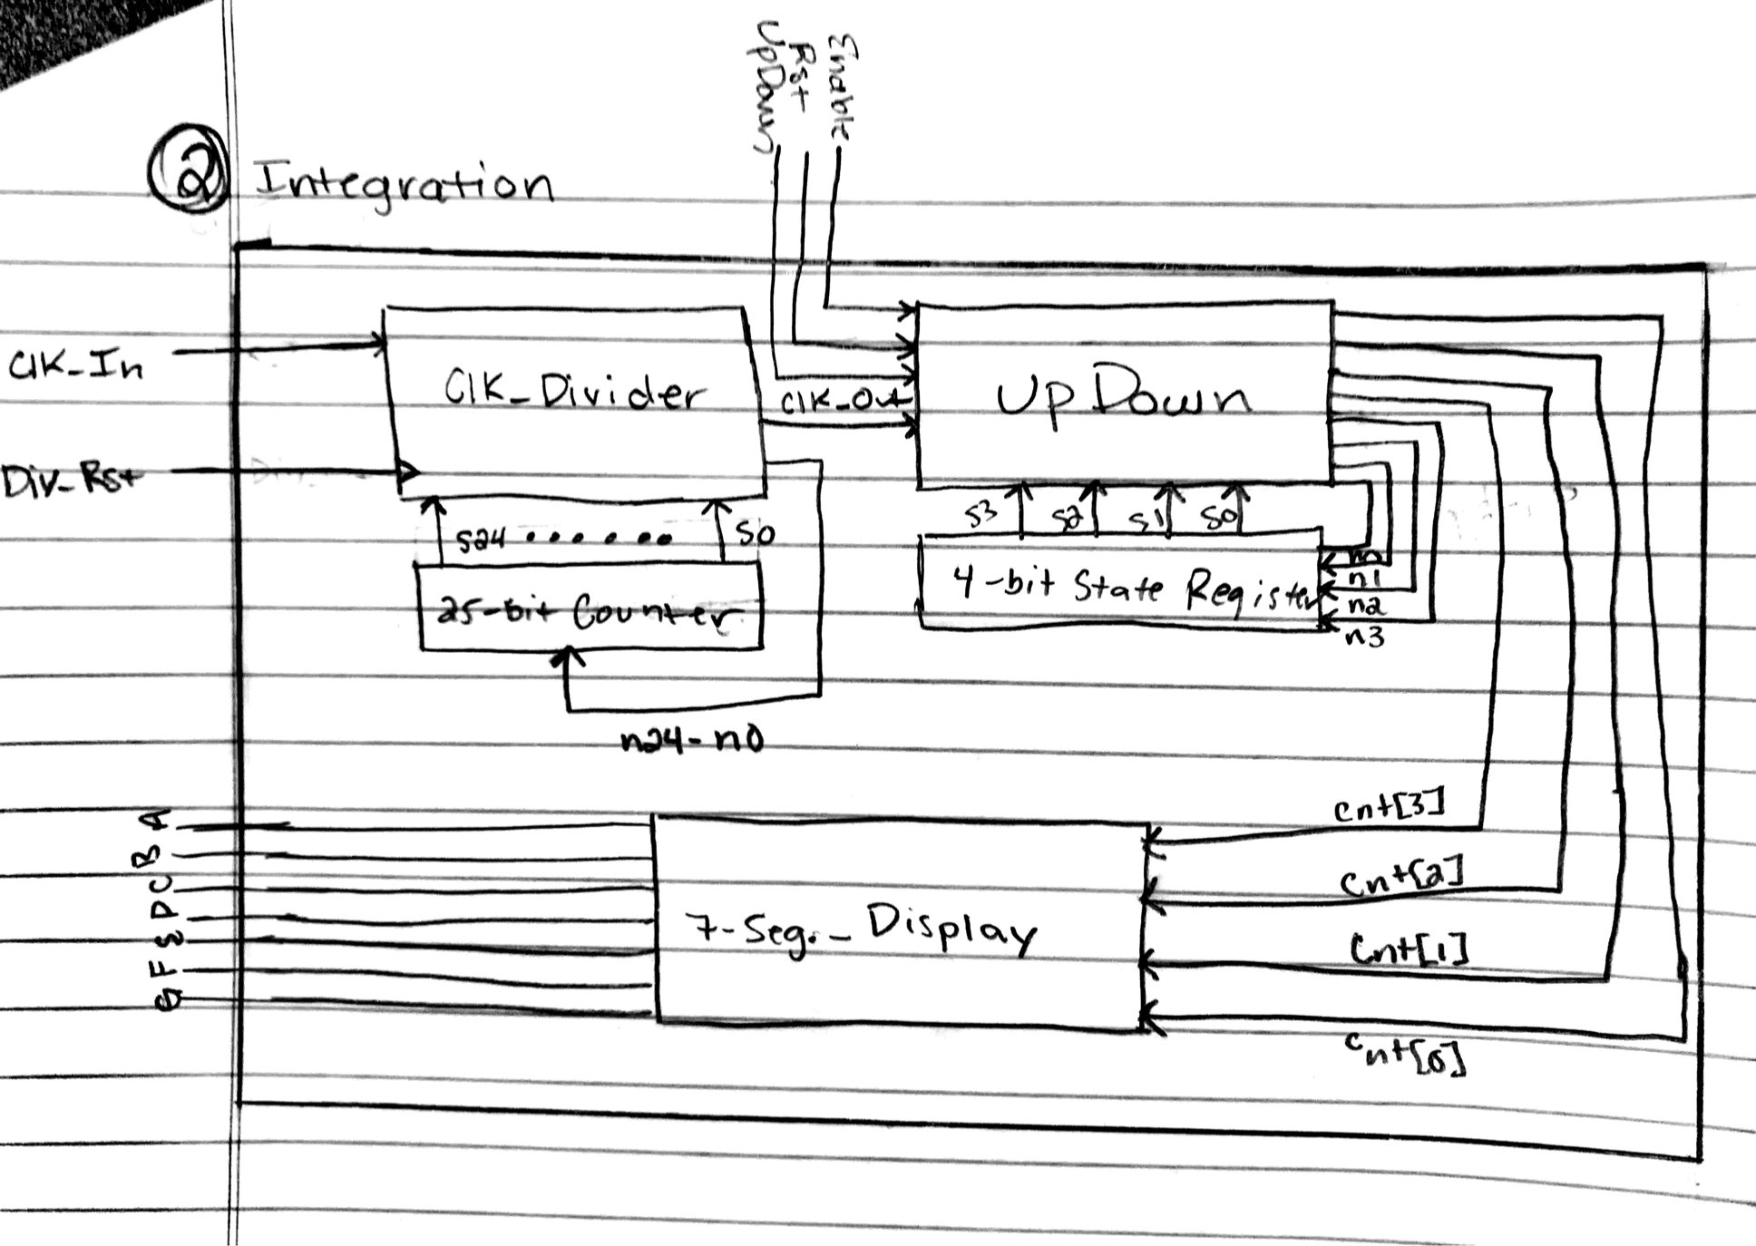
\includegraphics[scale=.5]{Prelab_7-page2.pdf}
			\end{center}
				\paragraph*{}If we compare this controller design to the previous lab, we can see that it is mostly the same design, with the addition of the 7 segment display.  
				The large difference is connecting the 4 state register of UpDown to the input
				of seven segment display. 
\newpage
	\subsection*{UpDown}
		\textbf{Behavioral Module Code}
		\begin{Verbatim}[frame=single, fontsize=\small]
`timescale 1ns / 1ps
////////////////////////////////////////////////////////////////////////////////
// Engineer:      Zachary Davis & Ryan Cruz
// 
// Create Date:    11:24:41 10/13/2017 
// Design Name:    UpDown_tb
// Module Name:    UpDown  
// Description:    Uses switches to control the seven segment display by 
//                 counting up or down on the rising edge of a clock cycle.
//						 
////////////////////////////////////////////////////////////////////////////////
module UpDown(Clk_Out, Rst, Enable, UpDown, Count);
	input Clk_Out, Rst, Enable, UpDown;
	output reg [3:0] Count = 4'b0000;
	
	always @ (posedge Clk_Out)
		begin
		if (Rst == 4'b0001)
			Count <= 4'b0000;
		else if (Enable == 4'b0000)
			Count <= Count;
		else
			begin
			if (UpDown == 4'b0001)
				begin
				if (Count == 4'b1111)
					Count <= 4'b0000;
				else
					Count <= Count + 4'b0001;
				end
			else
				begin
				if (Count == 4'b0000)
					Count <= 4'b1111;
				else
					Count <= Count - 4'b0001;
				end
		end
	end
endmodule
		\end{Verbatim}
		\paragraph*{}
			This is the code that stems from the FSM in the prelab.  No matter what is Rst is 
			high go to the Zero state, etc.  It follows the logic explained above.
		\newpage
		\flushleft
		\textbf{Test Bench Code}
		\begin{Verbatim}[frame=single, fontsize=\small]
`timescale 1ns / 1ps
////////////////////////////////////////////////////////////////////////////////
// Engineer:      Zachary Davis & Ryan Cruz
// 
// Create Date:    11:24:41 10/13/2017 
// Design Name:    UpDown_tb
// Module Name:    UpDown  
// Description:    Uses switches to control the seven segment display by 
//                 counting up or down on the rising edge of a clock cycle.
//						 
////////////////////////////////////////////////////////////////////////////////
module UpDown_tb();
	reg Clk_Out_t, Rst_t, UpDown_t, Enable_t;
	wire [3:0] Count_t;
	
	UpDown UpDown_1(Clk_Out_t, Rst_t, Enable_t, UpDown_t, Count_t);
	
	initial
	Clk_Out_t <= 0;
	
	always
	#10 Clk_Out_t <= ~Clk_Out_t;
	
	initial begin
	UpDown_t <= 0; Rst_t <= 0; Enable_t <= 0;
	@(posedge Clk_Out_t);
	@(posedge Clk_Out_t);
	@(posedge Clk_Out_t);
	@(posedge Clk_Out_t);
	UpDown_t <= 1; Rst_t <= 0; Enable_t <= 1;
	@(posedge Clk_Out_t);
	@(posedge Clk_Out_t);
	@(posedge Clk_Out_t);
	@(posedge Clk_Out_t);
	@(posedge Clk_Out_t);
	@(posedge Clk_Out_t);
	UpDown_t <= 0; Rst_t <= 0; Enable_t <= 1;
	@(posedge Clk_Out_t);
	@(posedge Clk_Out_t);
	@(posedge Clk_Out_t);
	@(posedge Clk_Out_t);
	@(posedge Clk_Out_t);
	@(posedge Clk_Out_t);
	@(posedge Clk_Out_t);
	Enable_t <= 0;
	@(posedge Clk_Out_t);
	@(posedge Clk_Out_t);
	Enable_t <= 1;
	@(posedge Clk_Out_t);
	@(posedge Clk_Out_t);	
	@(posedge Clk_Out_t);
	Rst_t <= 1;
	end
endmodule
		\end{Verbatim}
		\paragraph*{}
			We used the test bench to test many, but not all the use cases from the UpDown.v.  
			What we are doing is explained more in depth below with its wave form.

	\subsection*{SevenSegmentDisplay}
	\textbf{Behavioral Module Code}

		\begin{Verbatim}[frame=single, fontsize=\small]
`timescale 1ns / 1ps
////////////////////////////////////////////////////////////////////////////////
// Engineer:       Zachary Davis & Ryan Cruz
// 
// Create Date:    11:24:41 10/13/2017 
// Design Name:    Seven_Segment_Display
// Module Name:    Seven_Segment_Display  
// Description:    Displays the numbers 0-15 in hexidecimal on and LED display
//						 
////////////////////////////////////////////////////////////////////////////////
module Seven_Segment_Display(In, A, B, C, D, E, F, G);
	input [3:0] In;
	output A, B, C, D, E, F, G;
	reg A, B, C, D, E, F, G;
	
	always @ (In[3], In[2], In[1], In[0])
	begin
		if (In[3] == 0 && In[2] == 0 && In[1] == 0 && In[0] == 0)
		begin
		A <= 1;
		B <= 1;
		C <= 1;
		D <= 1;
		E <= 1;
		F <= 1;
		G <= 0;
		end
		else if (In[3] == 0 && In[2] == 0 && In[1] == 0 && In[0] == 1)
		begin
		A <= 0;
		B <= 1;
		C <= 1;
		D <= 0;
		E <= 0;
		F <= 0;
		G <= 0;
		end
		else if (In[3] == 0 && In[2] == 0 && In[1] == 1 && In[0] == 0)
		begin
		A <= 1;
		B <= 1;
		C <= 0;
		D <= 1;
		E <= 1;
		F <= 0;
		G <= 1;
		end
		else if (In[3] == 0 && In[2] == 0 && In[1] == 1 && In[0] == 1)
		begin
		A <= 1;
		B <= 1;
		C <= 1;
		D <= 1;
		E <= 0;
		F <= 0;
		G <= 1;
		end
		else if (In[3] == 0 && In[2] == 1 && In[1] == 0 && In[0] == 0)
		begin
		A <= 0;
		B <= 1;
		C <= 1;
		D <= 0;
		E <= 0;
		F <= 1;
		G <= 1;
		end
		else if (In[3] == 0 && In[2] == 1 && In[1] == 0 && In[0] == 1)
		begin
		A <= 1;
		B <= 0;
		C <= 1;
		D <= 1;
		E <= 0;
		F <= 1;
		G <= 1;
		end
		else if (In[3] == 0 && In[2] == 1 && In[1] == 1 && In[0] == 0)
		begin
		A <= 1;
		B <= 0;
		C <= 1;
		D <= 1;
		E <= 1;
		F <= 1;
		G <= 1;
		end
		else if (In[3] == 0 && In[2] == 1 && In[1] == 1 && In[0] == 1)
		begin
		A <= 1;
		B <= 1;
		C <= 1;
		D <= 0;
		E <= 0;
		F <= 0;
		G <= 0;
		end
		else if (In[3] == 1 && In[2] == 0 && In[1] == 0 && In[0] == 0)
		begin
		A <= 1;
		B <= 1;
		C <= 1;
		D <= 1;
		E <= 1;
		F <= 1;
		G <= 1;
		end
		else if (In[3] == 1 && In[2] == 0 && In[1] == 0 && In[0] == 1)
		begin
		A <= 1;
		B <= 1;
		C <= 1;
		D <= 1;
		E <= 0;
		F <= 1;
		G <= 1;
		end
		else if (In[3] == 1 && In[2] == 0 && In[1] == 1 && In[0] == 0)
		begin
		A <= 1;
		B <= 1;
		C <= 1;
		D <= 0;
		E <= 1;
		F <= 1;
		G <= 1;
		end
		else if (In[3] == 1 && In[2] == 0 && In[1] == 1 && In[0] == 1)
		begin
		A <= 0;
		B <= 0;
		C <= 1;
		D <= 1;
		E <= 1;
		F <= 1;
		G <= 1;
		end
		else if (In[3] == 1 && In[2] == 1 && In[1] == 0 && In[0] == 0)
		begin
		A <= 1;
		B <= 0;
		C <= 0;
		D <= 1;
		E <= 1;
		F <= 1;
		G <= 0;
		end
		else if (In[3] == 1 && In[2] == 1 && In[1] == 0 && In[0] == 1)
		begin
		A <= 0;
		B <= 1;
		C <= 1;
		D <= 1;
		E <= 1;
		F <= 0;
		G <= 1;
		end
		else if (In[3] == 1 && In[2] == 1 && In[1] == 1 && In[0] == 0)
		begin
		A <= 1;
		B <= 0;
		C <= 0;
		D <= 1;
		E <= 1;
		F <= 1;
		G <= 1;
		end
		else
		begin
		A <= 1;
		B <= 0;
		C <= 0;
		D <= 0;
		E <= 1;
		F <= 1;
		G <= 1;
		end
	end
endmodule
		\end{Verbatim}
		\paragraph*{}
			This is the logic from lab 3 earlier this semester.  However, we chose back then not 
			to use conidtion logic and we really paid the price this week.  Rather than bandaid 
			it all together we entirely rewrote this file from what we turned in in lab 3.  
			Functionally it works exactly the same it is just far more readable and more 
			compatable with a state register input.
		\vspace{1cm}

	\textbf{Test Bench Code}
		\begin{Verbatim}[frame=single, fontsize=\small]
`timescale 1ns / 1ps
////////////////////////////////////////////////////////////////////////////////
// Engineer:       Zachary Davis, Ryan Cruz
// 
// Create Date:    12:28:46 09/22/2017 
// Module Name:    Seven_Segment_Display 
// Project Name: 
// Target Devices: Sparten 3E
// Description:    Displays the numbers 0-15 in hexidecimal on and LED display
//
////////////////////////////////////////////////////////////////////////////////
module Seven_Segment_Display_tb();

	reg [3:0] In;
	wire A_t, B_t,C_t, D_t, E_t, F_t, G_t;

	Seven_Segment_Display Seven_Segment_Display_1
	(In, A_t, B_t,C_t, D_t, E_t, F_t, G_t);
	
	initial
	begin
	
	//Case 0
	In <= 4'b0000;
	#1 $display("");
	#1 $display("Case 0: ");
	#1 $display("A_t = %b", A_t);
	#1 $display("B_t = %b", B_t);
	#1 $display("C_t = %b", C_t);
	#1 $display("D_t = %b", D_t);
	#1 $display("E_t = %b", E_t);
	#1 $display("F_t = %b", F_t);
	#1 $display("G_t = %b", G_t);
	
	//Case 1
In <= 4'b0001;
	#1 $display("");
	#1 $display("Case 1: ");
	#1 $display("A_t = %b", A_t);
	#1 $display("B_t = %b", B_t);
	#1 $display("C_t = %b", C_t);
	#1 $display("D_t = %b", D_t);
	#1 $display("E_t = %b", E_t);
	#1 $display("F_t = %b", F_t);
	#1 $display("G_t = %b", G_t);
	
	//Case 2
In <= 4'b0010;
	#1 $display("");
	#1 $display("Case 2: ");
	#1 $display("A_t = %b", A_t);
	#1 $display("B_t = %b", B_t);
	#1 $display("C_t = %b", C_t);
	#1 $display("D_t = %b", D_t);
	#1 $display("E_t = %b", E_t);
	#1 $display("F_t = %b", F_t);
	#1 $display("G_t = %b", G_t);
	
	//Case 3
In <= 4'b0011;
	#1 $display("");
	#1 $display("Case 3: ");
	#1 $display("A_t = %b", A_t);
	#1 $display("B_t = %b", B_t);
	#1 $display("C_t = %b", C_t);
	#1 $display("D_t = %b", D_t);
	#1 $display("E_t = %b", E_t);
	#1 $display("F_t = %b", F_t);
	#1 $display("G_t = %b", G_t);
	
	//Case 4
In <= 4'b0100;
	#1 $display("");
	#1 $display("Case 4: ");
	#1 $display("A_t = %b", A_t);
	#1 $display("B_t = %b", B_t);
	#1 $display("C_t = %b", C_t);
	#1 $display("D_t = %b", D_t);
	#1 $display("E_t = %b", E_t);
	#1 $display("F_t = %b", F_t);
	#1 $display("G_t = %b", G_t);
	
	//Case 5
In <= 4'b0101;
	#1 $display("");
	#1 $display("Case 5: ");
	#1 $display("A_t = %b", A_t);
	#1 $display("B_t = %b", B_t);
	#1 $display("C_t = %b", C_t);
	#1 $display("D_t = %b", D_t);
	#1 $display("E_t = %b", E_t);
	#1 $display("F_t = %b", F_t);
	#1 $display("G_t = %b", G_t);
	
	//Case 6
In <= 4'b0110;
	#1 $display("");
	#1 $display("Case 6: ");
	#1 $display("A_t = %b", A_t);
	#1 $display("B_t = %b", B_t);
	#1 $display("C_t = %b", C_t);
	#1 $display("D_t = %b", D_t);
	#1 $display("E_t = %b", E_t);
	#1 $display("F_t = %b", F_t);
	#1 $display("G_t = %b", G_t);
	
	//Case 7
In <= 4'b0111;
	#1 $display("");
	#1 $display("Case 7: ");
	#1 $display("A_t = %b", A_t);
	#1 $display("B_t = %b", B_t);
	#1 $display("C_t = %b", C_t);
	#1 $display("D_t = %b", D_t);
	#1 $display("E_t = %b", E_t);
	#1 $display("F_t = %b", F_t);
	#1 $display("G_t = %b", G_t);
	
	//Case 8
In <= 4'b1000;
	#1 $display("");
	#1 $display("Case 8: ");
	#1 $display("A_t = %b", A_t);
	#1 $display("B_t = %b", B_t);
	#1 $display("C_t = %b", C_t);
	#1 $display("D_t = %b", D_t);
	#1 $display("E_t = %b", E_t);
	#1 $display("F_t = %b", F_t);
	#1 $display("G_t = %b", G_t);
	
	//Case 9
	In <= 4'b1001;
	#1 $display("");
	#1 $display("Case 9: ");
	#1 $display("A_t = %b", A_t);
	#1 $display("B_t = %b", B_t);
	#1 $display("C_t = %b", C_t);
	#1 $display("D_t = %b", D_t);
	#1 $display("E_t = %b", E_t);
	#1 $display("F_t = %b", F_t);
	#1 $display("G_t = %b", G_t);
	
	//Case 10
	In <= 4'b1010;
	#1 $display("");
	#1 $display("Case 10: ");
	#1 $display("A_t = %b", A_t);
	#1 $display("B_t = %b", B_t);
	#1 $display("C_t = %b", C_t);
	#1 $display("D_t = %b", D_t);
	#1 $display("E_t = %b", E_t);
	#1 $display("F_t = %b", F_t);
	#1 $display("G_t = %b", G_t);
	
	//Case 11
	In <= 4'b1011;
	#1 $display("");
	#1 $display("Case 11: ");
	#1 $display("A_t = %b", A_t);
	#1 $display("B_t = %b", B_t);
	#1 $display("C_t = %b", C_t);
	#1 $display("D_t = %b", D_t);
	#1 $display("E_t = %b", E_t);
	#1 $display("F_t = %b", F_t);
	#1 $display("G_t = %b", G_t);
	
	//Case 12
	In <= 4'b1100;
	#1 $display("");
	#1 $display("Case 12: ");
	#1 $display("A_t = %b", A_t);
	#1 $display("B_t = %b", B_t);
	#1 $display("C_t = %b", C_t);
	#1 $display("D_t = %b", D_t);
	#1 $display("E_t = %b", E_t);
	#1 $display("F_t = %b", F_t);
	#1 $display("G_t = %b", G_t);
	
	//Case 13
	In <= 4'b1101;
	#1 $display("");
	#1 $display("Case 13: ");
	#1 $display("A_t = %b", A_t);
	#1 $display("B_t = %b", B_t);
	#1 $display("C_t = %b", C_t);
	#1 $display("D_t = %b", D_t);
	#1 $display("E_t = %b", E_t);
	#1 $display("F_t = %b", F_t);
	#1 $display("G_t = %b", G_t);
	
	//Case 14
	In <= 4'b1110;
	#1 $display("");
	#1 $display("Case 14: ");
	#1 $display("A_t = %b", A_t);
	#1 $display("B_t = %b", B_t);
	#1 $display("C_t = %b", C_t);
	#1 $display("D_t = %b", D_t);
	#1 $display("E_t = %b", E_t);
	#1 $display("F_t = %b", F_t);
	#1 $display("G_t = %b", G_t);
	
	//Case 15
	In <= 4'b1111;
	#1 $display("");
	#1 $display("Case 15: ");
	#1 $display("A_t = %b", A_t);
	#1 $display("B_t = %b", B_t);
	#1 $display("C_t = %b", C_t);
	#1 $display("D_t = %b", D_t);
	#1 $display("E_t = %b", E_t);
	#1 $display("F_t = %b", F_t);
	#1 $display("G_t = %b", G_t);

	end
endmodule
		\end{Verbatim}
		\paragraph*{}
			This is our testbench for seven segment display.  What exactly is happening here is 
			explained below with its waveform.
\newpage
\subsection*{Clock Divider}
	\textbf{Behavioral Module Code}

		\begin{Verbatim}[frame=single, fontsize=\small]
`timescale 1ns / 1ps
////////////////////////////////////////////////////////////////////////////////
// Engineer:       Zachary Davis & Ryan Cruz
// 
// Create Date:    11:24:41 10/13/2017 
// Design Name:    Thunderbird Turn Signal
// Module Name:    Clock_Divider_tb 
// Description:    A clock divider that divides 50 MHz into 1 Hz on the FPGA
//                 board.  Simulator.
//
////////////////////////////////////////////////////////////////////////////////
module Clock_Divider(Clk_In, Div_Rst, Clk_Out);
	input Clk_In, Div_Rst;
	output reg Clk_Out;
	reg [24:0] counter;
	
	always @(posedge Clk_In or posedge Div_Rst)
		begin
		if (Div_Rst == 1'b1)
			begin
			counter <= 0;
			Clk_Out <= 0;
			end
		else
			begin
			counter <= counter + 1;
			if (counter == 25_000_000) //25_000_000
				begin
				counter <= 0;
				Clk_Out <= ~Clk_Out;
				end
			end
		end
endmodule
		\end{Verbatim}
		\paragraph*{}
			This is the exact same code from a previous lab and does the exact same thing.  Its 
			purpose is to divide the 50mHz clock speed of the Sparten3E to 1 lowly Hz.
		\vspace{1cm}

	\newpage	
	\textbf{Test Bench Code}

		\begin{Verbatim}[frame=single, fontsize=\small]
`timescale 1ns / 1ps
////////////////////////////////////////////////////////////////////////////////
// Engineer:       Zachary Davis & Ryan Cruz
// 
// Create Date:    11:24:41 10/13/2017 
// Design Name:    Thunderbird Turn Signal
// Module Name:    Clock_Divider_tb 
// Description:    A clock divider that divides 50 MHz into 1 Hz on the FPGA
//                 board.  Simulator.
//
////////////////////////////////////////////////////////////////////////////////
module Clock_Divider_tb();
	reg Clk_In_t, Div_Rst_t;
	wire Clk_Out_t;
	
	Clock_Divider Clock_Divider_1(Clk_In_t, Div_Rst_t, Clk_Out_t);
	
	always
		begin
			Clk_In_t <= 1;
			#10;
			Clk_In_t <= 0;
			#10;
		end
	
	initial begin
		Div_Rst_t <= 0;
		#5;
		Div_Rst_t <= 1;
		#5;
		Div_Rst_t <= 0;
	end
endmodule
		\end{Verbatim}
		\paragraph*{}
			This is the testbench for the clock divider and it is altered for the simulation so 
			that it is usable.  This is explained further in the waveform below.

\newpage
\subsection*{Top Module}
	\textbf{Behavioral Module Code}

		\begin{Verbatim}[frame=single, fontsize=\small]
`timescale 1ns / 1ps
////////////////////////////////////////////////////////////////////////////////
// Engineer:       Zachary Davis & Ryan Cruz
// 
// Create Date:    12:29:15 10/20/2017 
// Design Name:    Seven Segment Display
// Module Name:    Top_Mod 
// Description:    Call on clock divider, seven segement display, and up down
//                 to combine the whole project.
//
////////////////////////////////////////////////////////////////////////////////
`timescale 1ns / 1ps

module Top_Mod(Clk_In, Rst, Enable, UpDown, A, B, C, D, E, F, G, Div_Rst);
	input Clk_In, Rst, Enable, UpDown, Div_Rst;
	output A, B, C, D, E, F, G;
	
	wire Clk_Out;
	wire [3:0] Count;

	Clock_Divider Clock_Divider_1 (Clk_In, Div_Rst, Clk_Out);
	UpDown UpDown_1 (Clk_Out, Rst, Enable, UpDown, Count);
	Seven_Segment_Display Seven_Segment_Display_1 (Count, A, B, C, D, E, F, G);
endmodule
		\end{Verbatim}
		\paragraph*{}
			This is the top module that calls all of the above as functions and connects them 
			together as shown in part two of the prelab.
		\vspace{1cm}

	\textbf{UCF}
		\begin{Verbatim}[frame=single, fontsize=\small]
NET "Clk_In" LOC = "C9";
NET "Rst" LOC = "K17" | PULLDOWN;
NET "Div_Rst" LOC = "D18" | PULLDOWN;
NET "Enable" LOC = "N17";
NET "UpDown" LOC = "H18";
NET "A" LOC = B4;
NET "B" LOC = A4;
NET "C" LOC = D5;
NET "D" LOC = C5;
NET "E" LOC = A6;
NET "F" LOC = B6;
NET "G" LOC = E7;
		\end{Verbatim}
		\paragraph*{}
			Assigning the four inputs to switches on the FPGA board as well as the clock.  It 
			also assigns the seven letters to a segment on the LED.

\section*{Experimental Results}
	
	\subsection*{Waveforms}
		\vspace{1cm}
		\begin{center}
			\textbf{Clock Divider Simulation}
			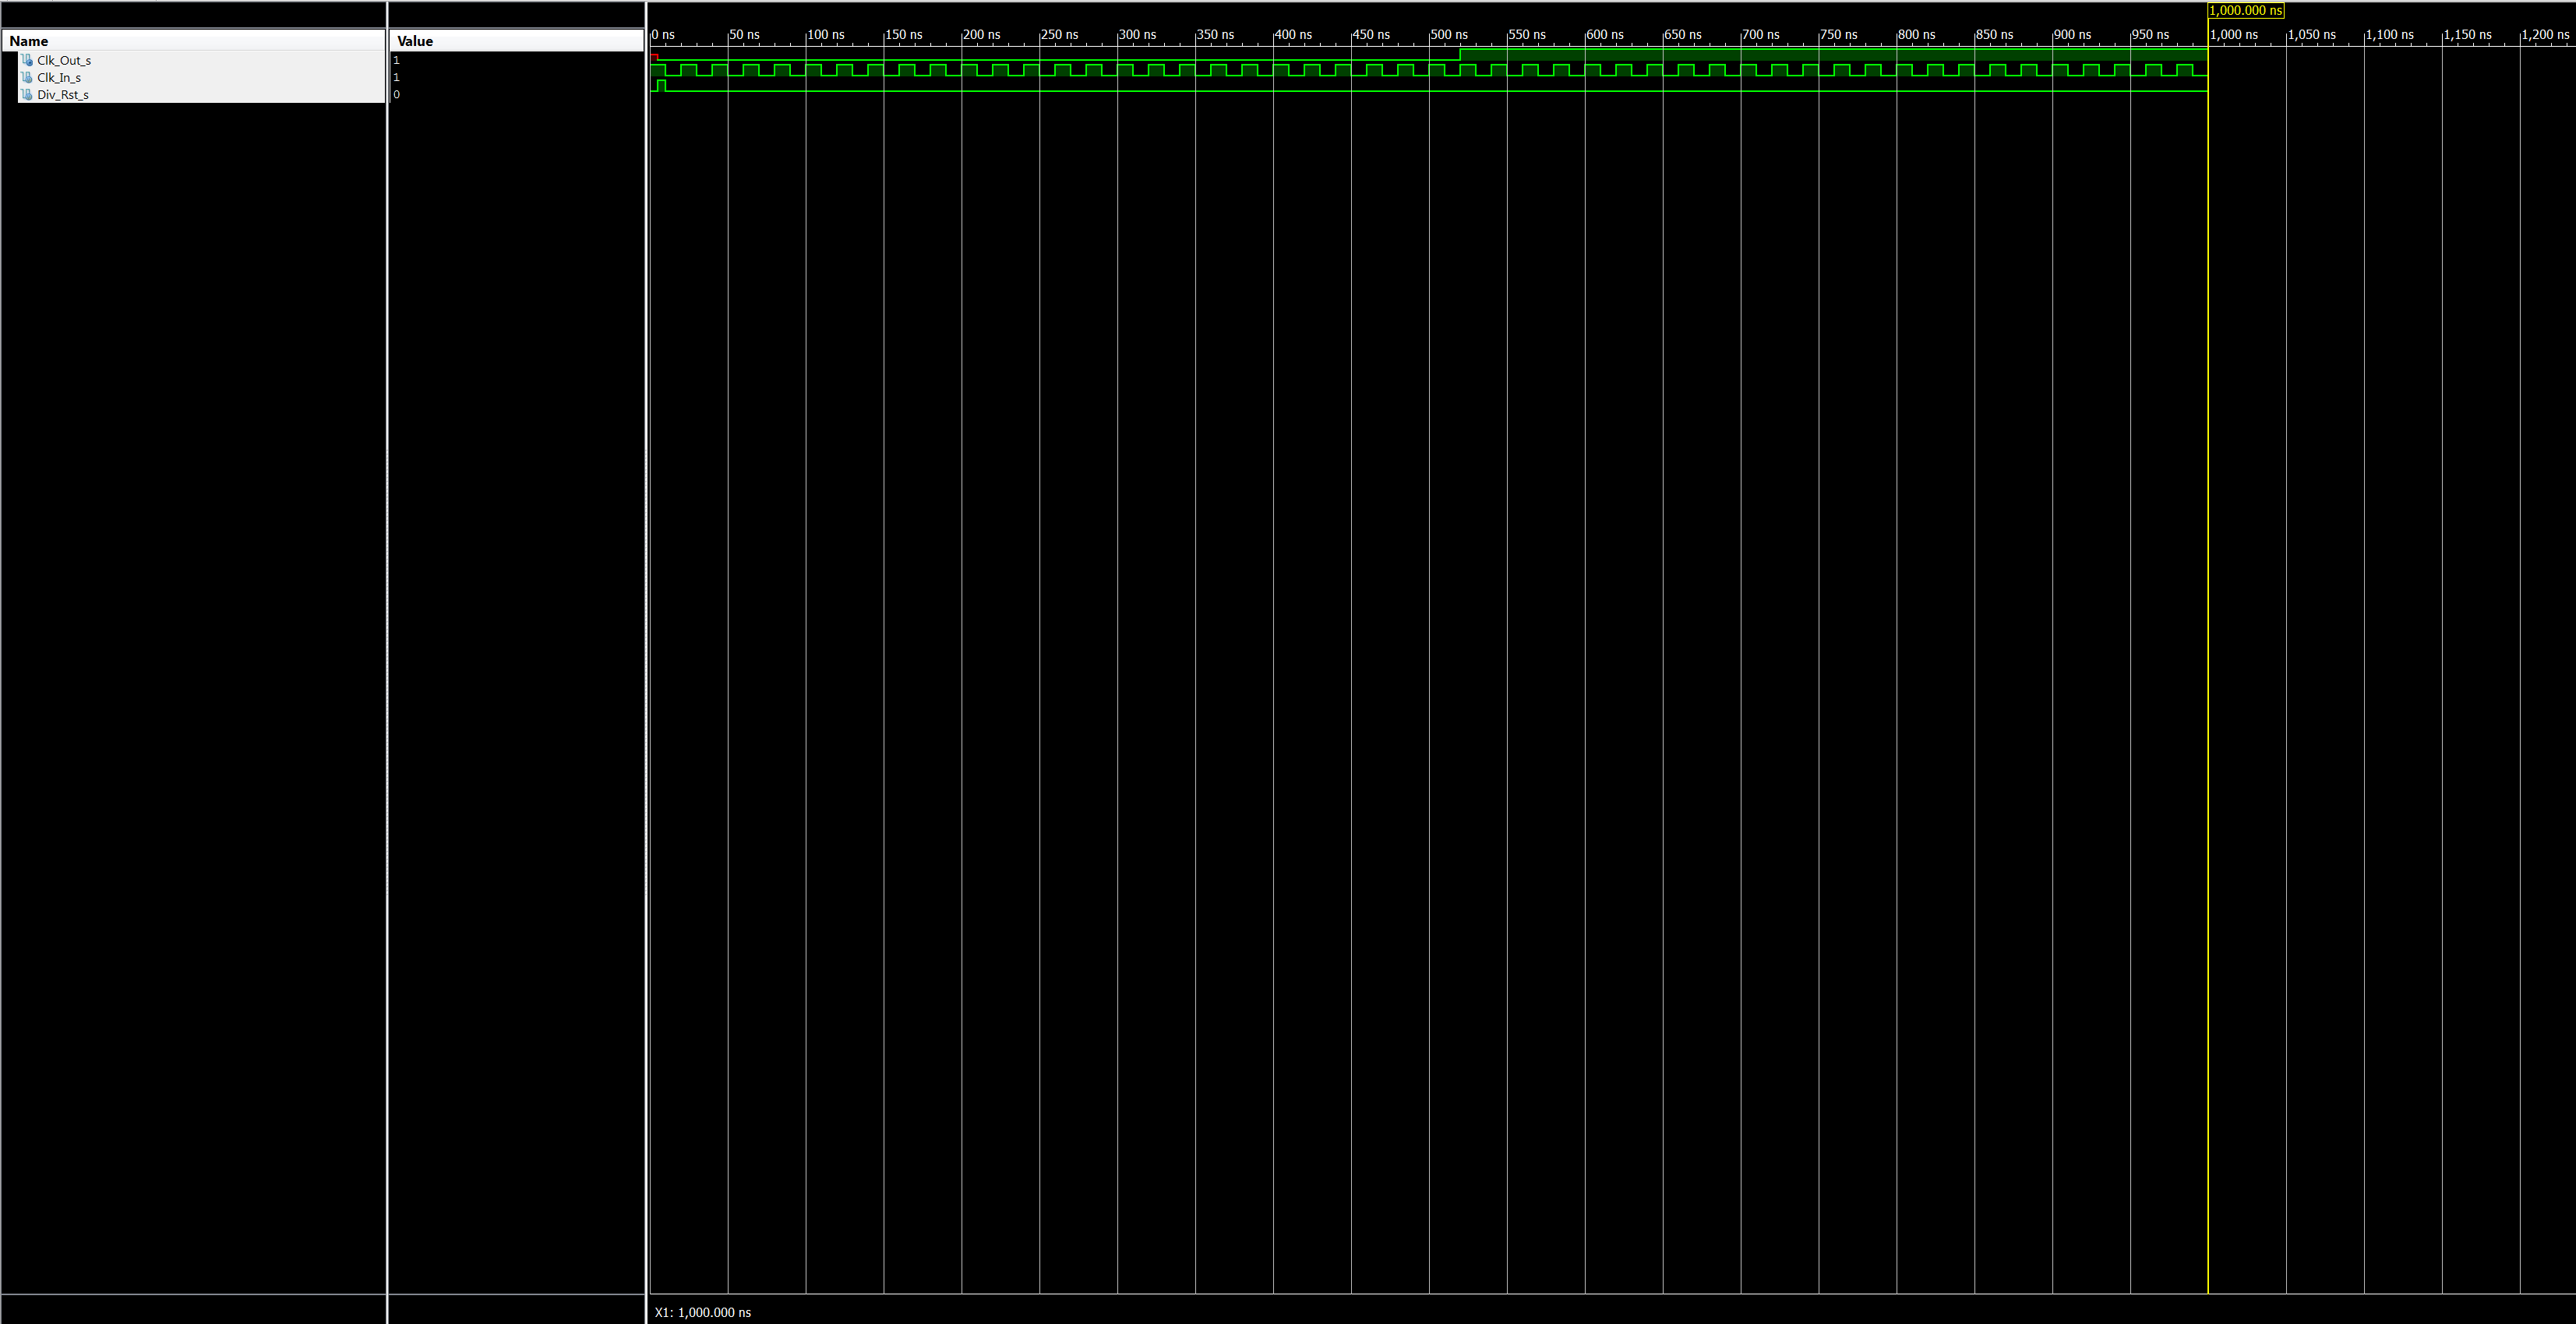
\includegraphics[scale=.28]{tb_1.PNG}
		\end{center}
			\paragraph*{}
				This code came straight from a previousl lab.  For the actual project we 
				intended for clock divider to take the 50mHz clock and divide it into a 1Hz 
				clock, but for the sake of the simulation we divided it into 1mHz clock so we 
				could actually see the result.
		\vspace{10cm}
		\begin{center}
			\textbf{UpDown Simulations}
			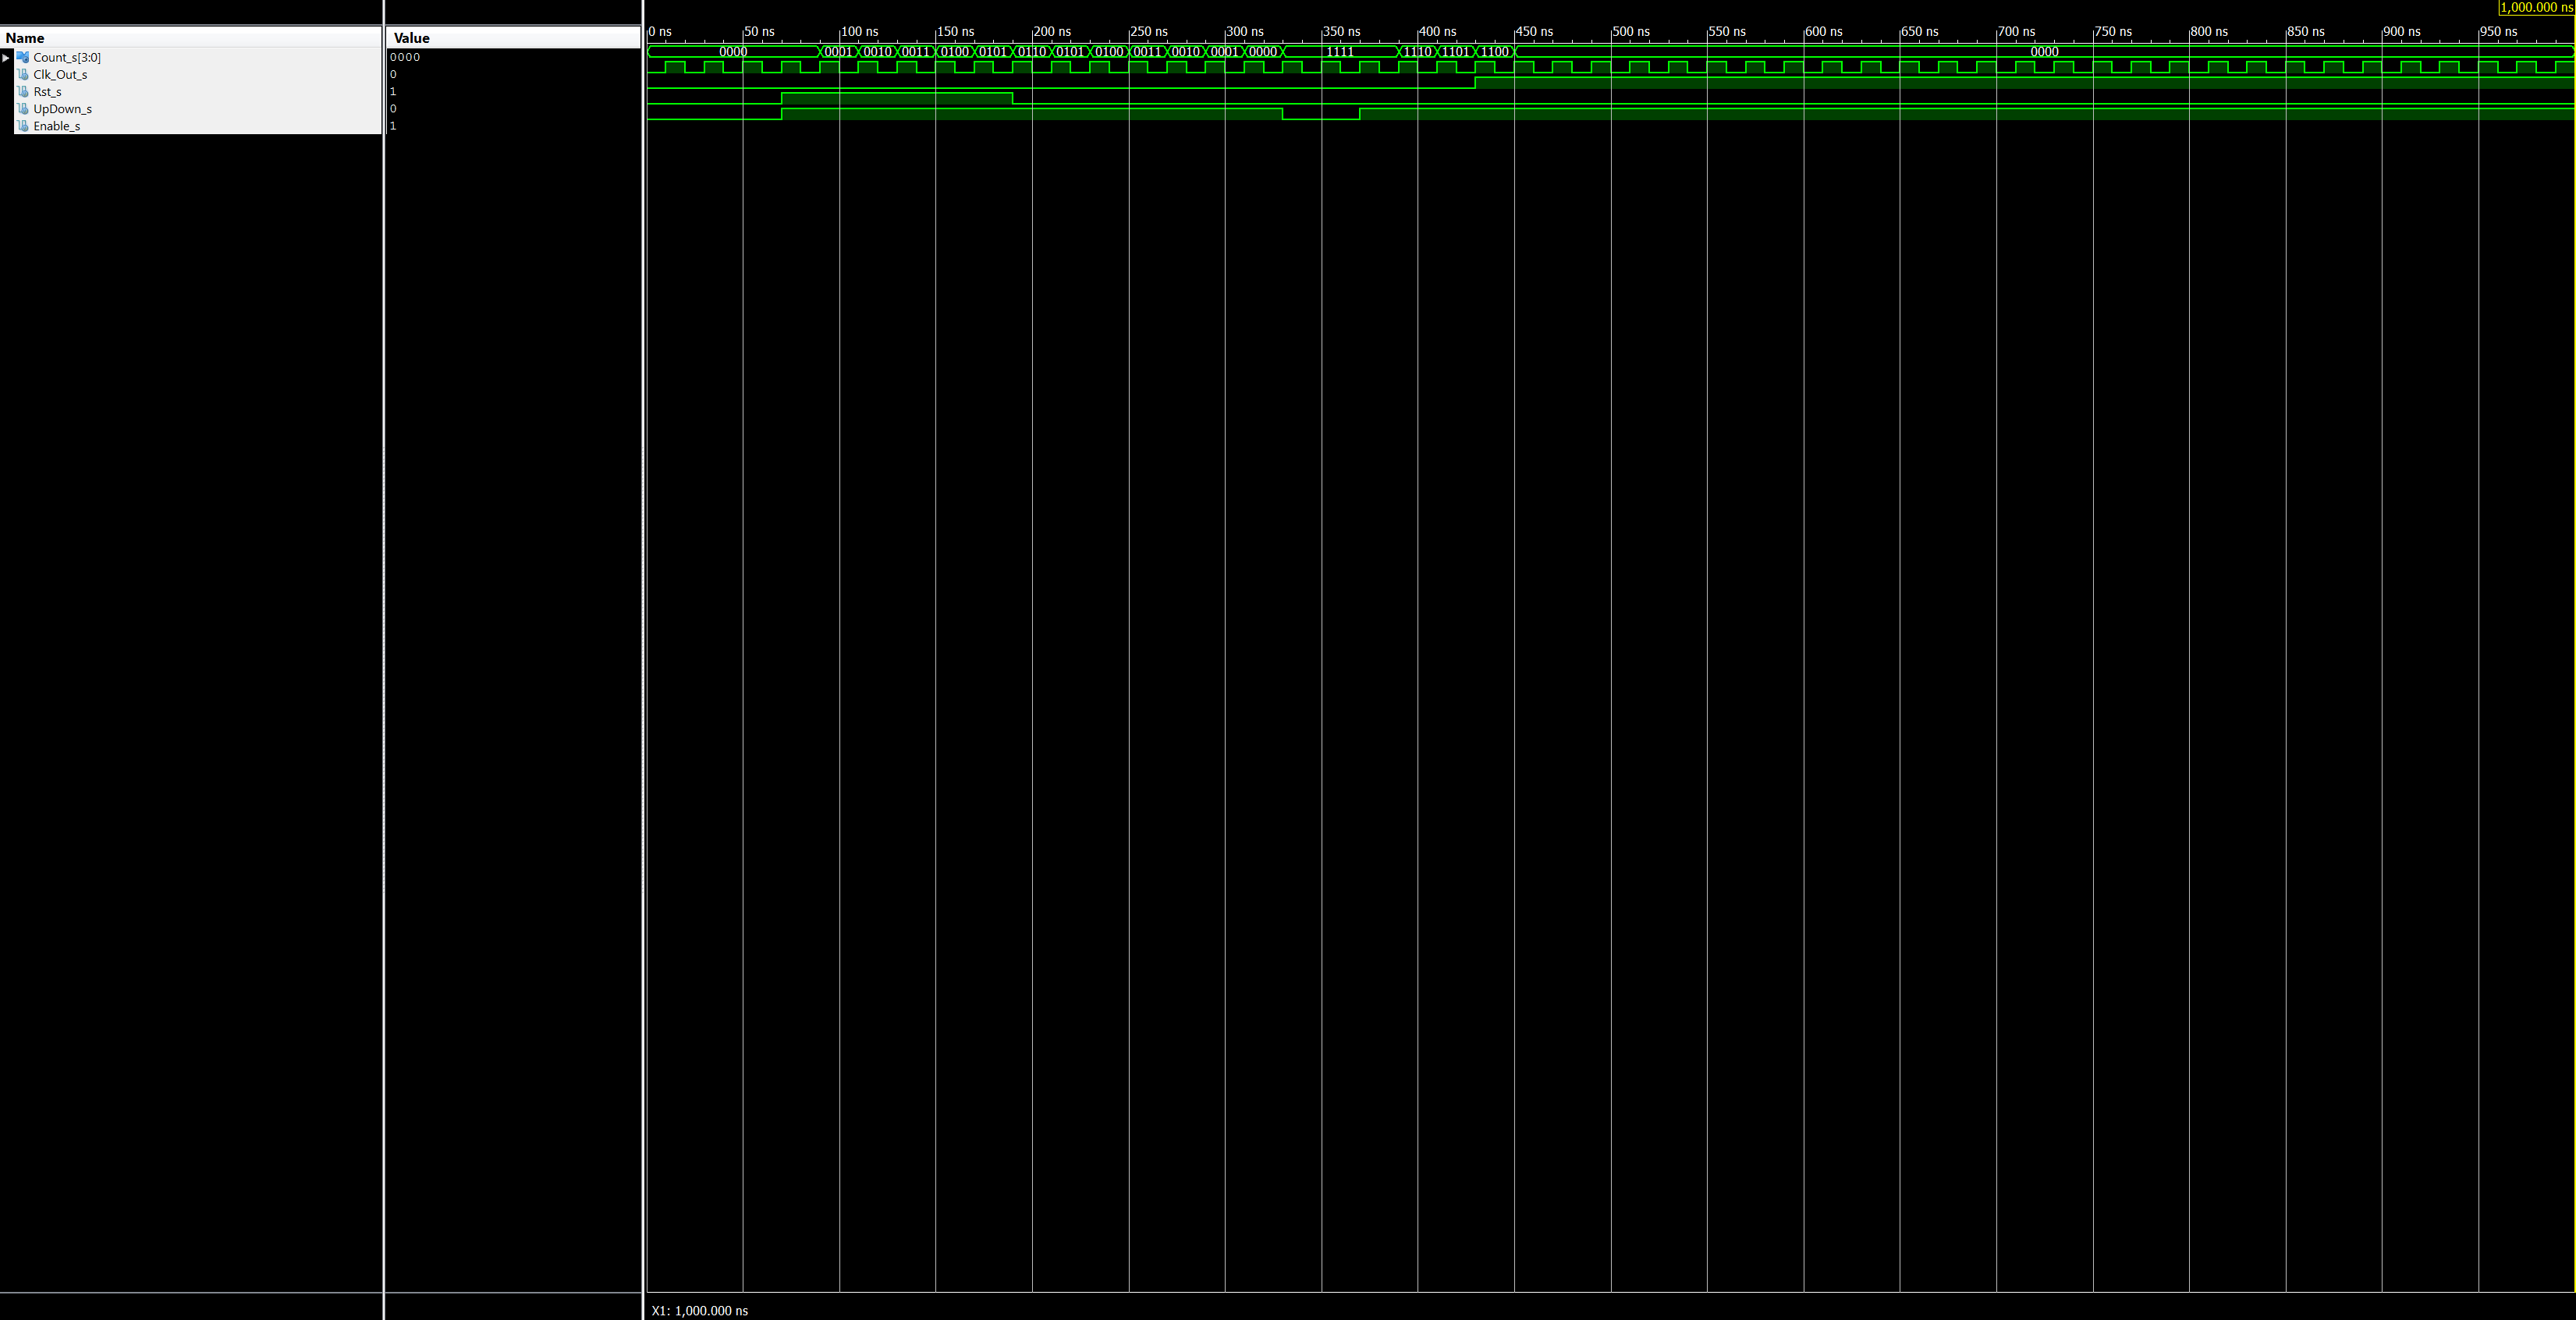
\includegraphics[scale=.28]{tb_2.PNG}
		\end{center}
			\paragraph*{}
				This simulation checks that UpDown counter acts as intended.  To do this we 
				checked all of the use cases we could come up with.  Initially no switch is
				high and our default case is 0.  From there UpDown and Enable are high which
				means the output should count up every clock cycle as it does.  Then just before 
				200ns we turn UpDown low and the outputs begin counting down.  Inbetween 300ns 
				and 350ns you can see it wrap from 0000 to 1111.  Also we turn Enable low which
				holds the output value at whatever it is.  Finally we turn Enable high and Rst 
				high to show that Rst returns it to 0000.  Enable does not actually need to be 
				high for this, which we did not show but we demonstrated in the demo.
		\vspace{10cm}
		\begin{center}
			\textbf{Seven Segment Display Simulation}
			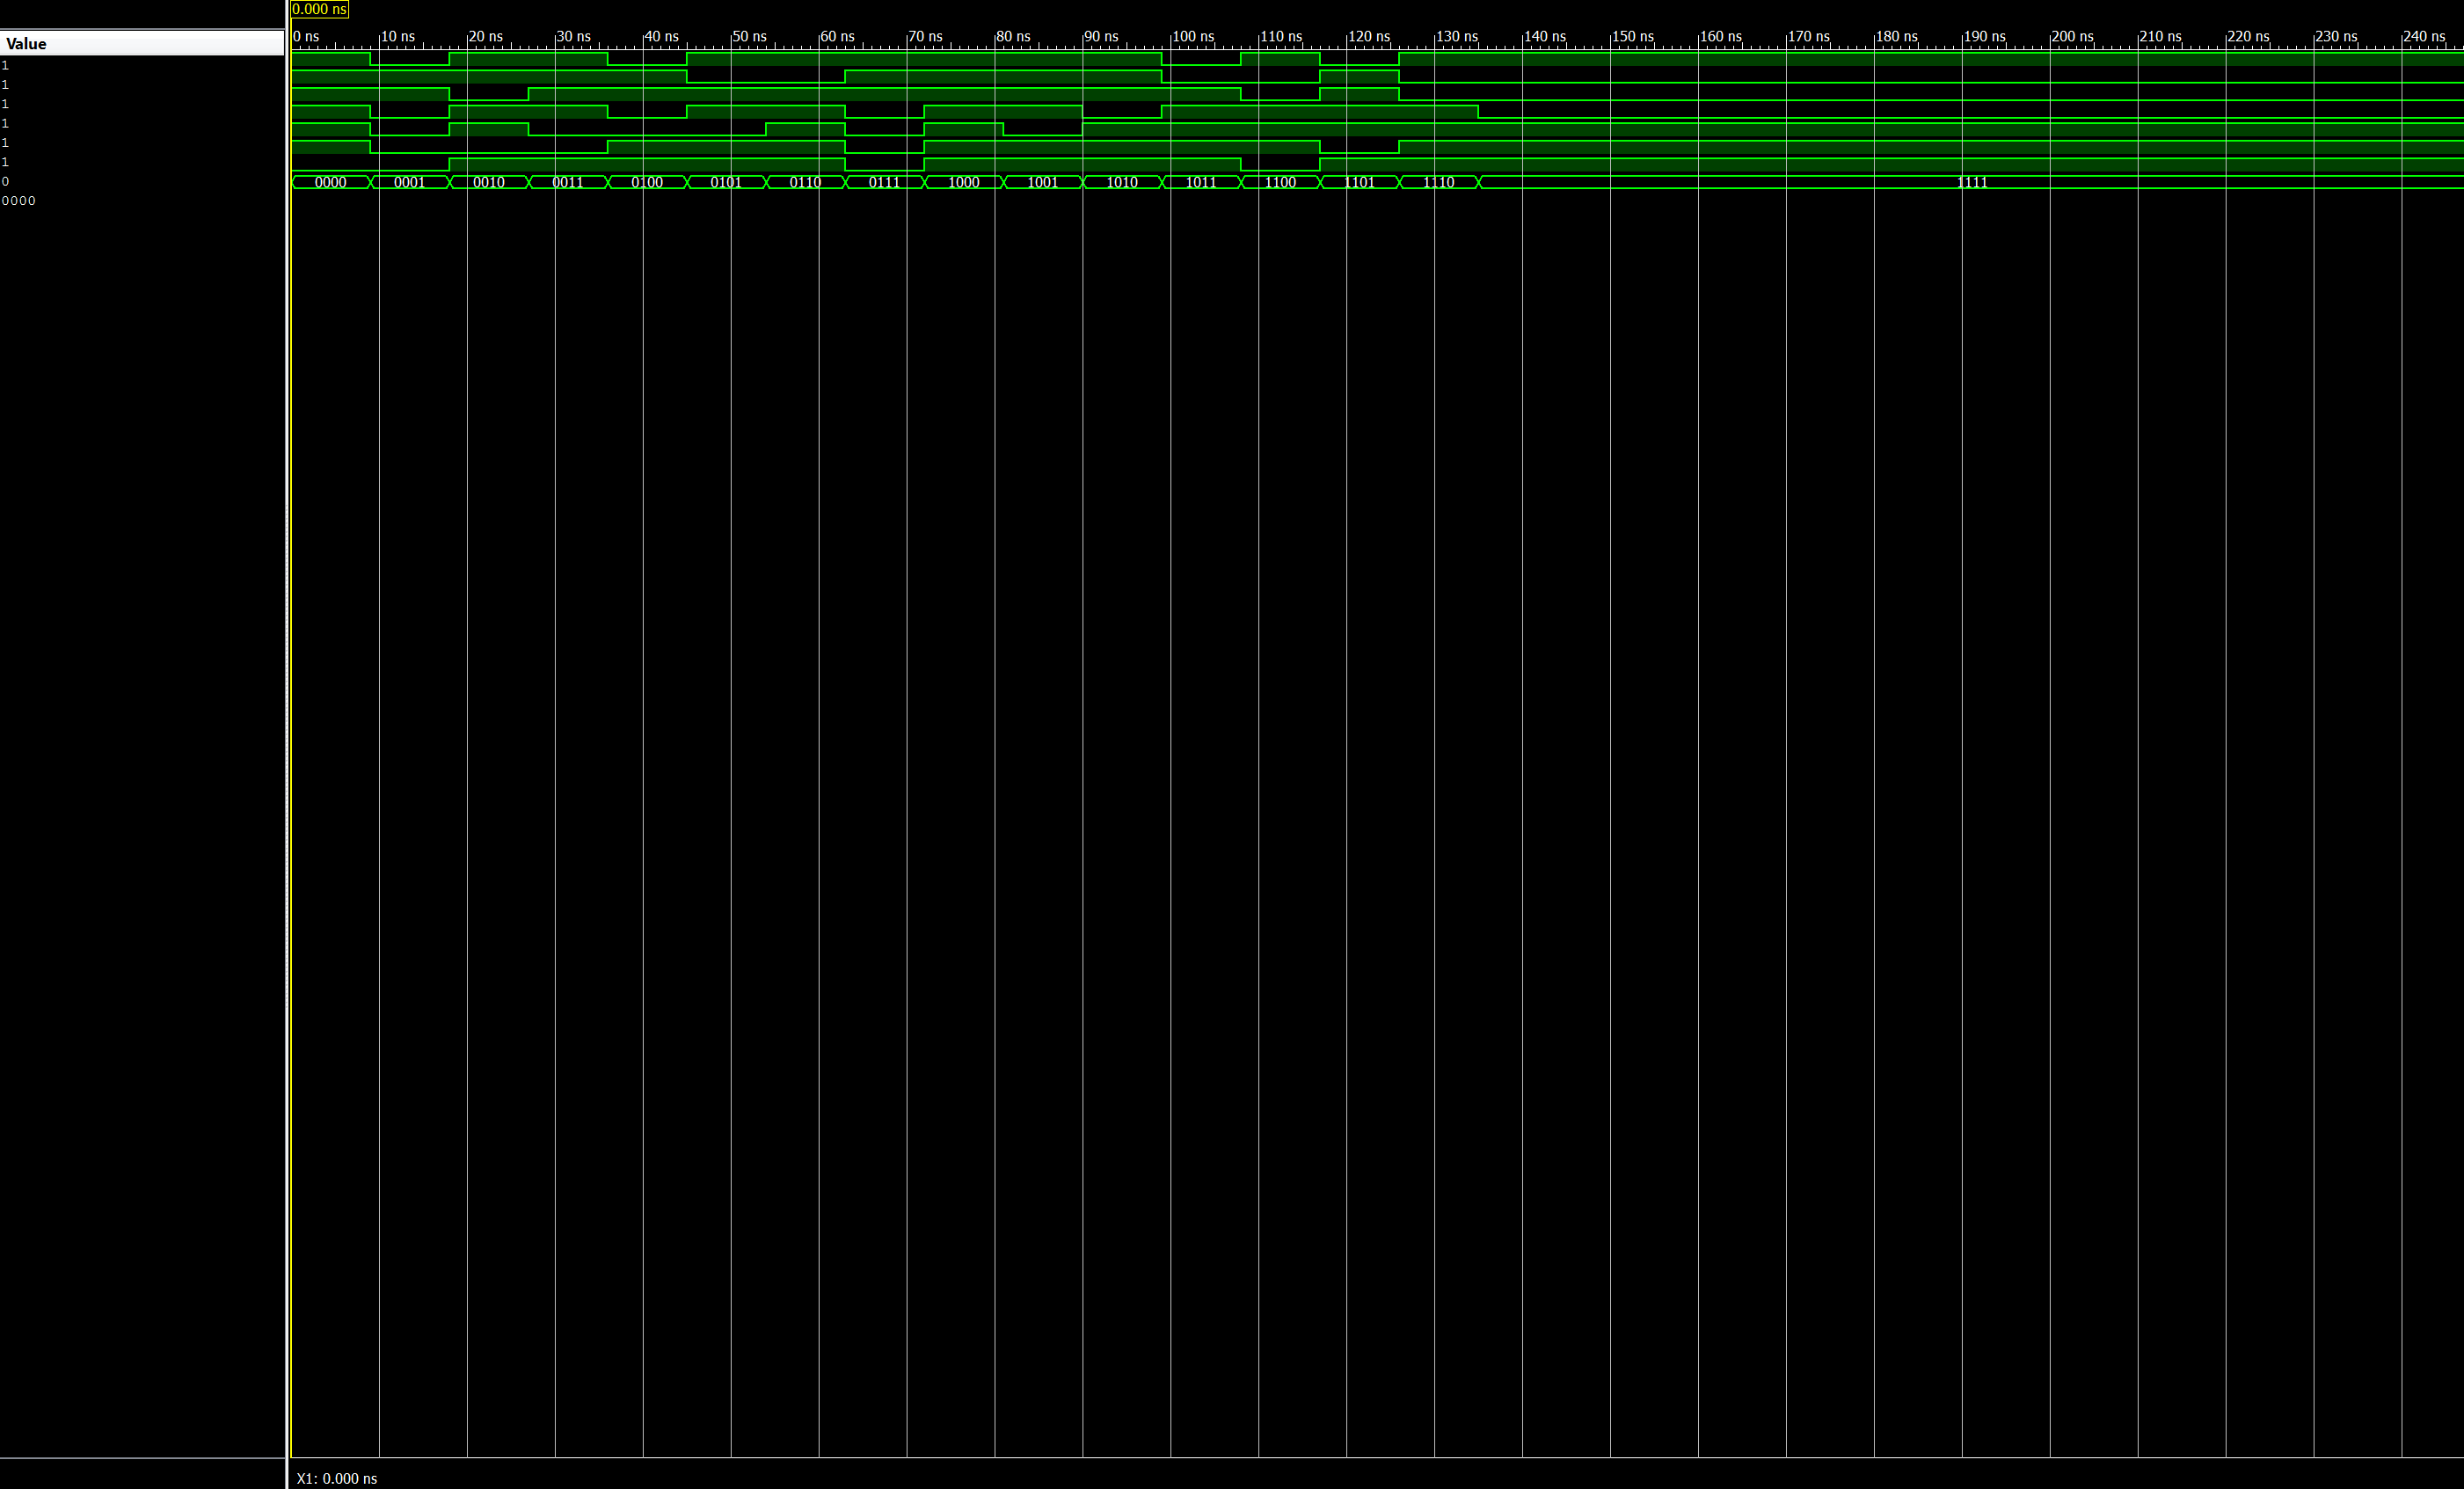
\includegraphics[scale=.3295]{tb_3.PNG}
		\end{center}
			\paragraph*{}
				This simulation shows all fifthteen posible cases for seven segment display.  The 
				simulation should look exactly the same as it did in lab three all though the way
				it is implemented was changed as explained above.  Either way the state register 
				is shown and the appropiate segments of the LED are high to form that digit.

\section*{Significance}
	This lab added another layer of complexity, introducing the concept of binary coded decimal and combining several topics from the previous labs, including clock division, displaying to the LED seven segment display, and binary/decimal/hex counting.  It as we said above also 
	stressed the value of behavioral logic as we had to change our previous design for seven 
	segment display.
			
\section*{Comments/Suggestions}
	\paragraph{}
		This lab is fine and builds up at a nice pace so that it does not feel to overwhelming, 
		but if I had to change anything it would be a mention that we are able to simplify our
		FSM's in the prelab they are getting very complex and repeatitive logic is overcrowding 
		the page like the RST switch.
		
\end{document}

